% This is "sig-alternate.tex" V2.1 April 2013
% This file should be compiled with V2.5 of "sig-alternate.cls" May 2012
%
% This example file demonstrates the use of the 'sig-alternate.cls'
% V2.5 LaTeX2e document class file. It is for those submitting
% articles to ACM Conference Proceedings WHO DO NOT WISH TO
% STRICTLY ADHERE TO THE SIGS (PUBS-BOARD-ENDORSED) STYLE.
% The 'sig-alternate.cls' file will produce a similar-looking,
% albeit, 'tighter' paper resulting in, invariably, fewer pages.
%
% ----------------------------------------------------------------------------------------------------------------
% This .tex file (and associated .cls V2.5) produces:
%       1) The Permission Statement
%       2) The Conference (location) Info information
%       3) The Copyright Line with ACM data
%       4) NO page numbers
%
% as against the acm_proc_article-sp.cls file which
% DOES NOT produce 1) thru' 3) above.
%
% Using 'sig-alternate.cls' you have control, however, from within
% the source .tex file, over both the CopyrightYear
% (defaulted to 200X) and the ACM Copyright Data
% (defaulted to X-XXXXX-XX-X/XX/XX).
% e.g.
% \CopyrightYear{2007} will cause 2007 to appear in the copyright line.
% \crdata{0-12345-67-8/90/12} will cause 0-12345-67-8/90/12 to appear in the copyright line.
%
% ---------------------------------------------------------------------------------------------------------------
% This .tex source is an example which *does* use
% the .bib file (from which the .bbl file % is produced).
% REMEMBER HOWEVER: After having produced the .bbl file,
% and prior to final submission, you *NEED* to 'insert'
% your .bbl file into your source .tex file so as to provide
% ONE 'self-contained' source file.
%
% ================= IF YOU HAVE QUESTIONS =======================
% Questions regarding the SIGS styles, SIGS policies and
% procedures, Conferences etc. should be sent to
% Adrienne Griscti (griscti@acm.org)
%
% Technical questions _only_ to
% Gerald Murray (murray@hq.acm.org)
% ===============================================================
%
% For tracking purposes - this is V2.0 - May 2012

\documentclass{sig-alternate-05-2015}

% *** CITATION PACKAGES ***
\usepackage{cite}

% *** MATH PACKAGES ***
\usepackage{amsmath}
\usepackage{svg}
\usepackage{amsfonts}

% *** PDF, URL AND HYPERLINK PACKAGES ***
\usepackage{url}
\usepackage{hyperref}
\usepackage{epigraph}

% *** ALGORITHM ***
\usepackage{algorithm}
\usepackage{algpseudocode}
\usepackage{booktabs}
\usepackage{enumitem}

% *** GRAPH***
\usepackage{graphics,graphicx}
\usepackage{pstricks,pst-node,pst-tree}
\usepackage{caption}

% *** FILLER TEXT ***
\usepackage{lipsum}

% *** STRIKEPUT ***
\usepackage{soul}

% *** To balance reference page ***
\usepackage{flushend}

% format

\usepackage{dblfloatfix}


\newcommand{\paragraphb}[1]{\vspace{0.03in}\noindent{\bf #1} }
\newcommand{\paragraphe}[1]{\vspace{0.03in}\noindent{\em #1} }
\newcommand{\paragraphbe}[1]{\vspace{0.03in}\noindent{\bf \em #1} }

\newcommand{\kevin}[1]{{\color{red}{#1}}}
\newcommand{\kevinc}[1]{{\color{red}\bf\em{[kevin: #1]}}}

\newcommand{\name}{DSSnet\xspace}
\newcommand{\Name}{DSSnet\xspace}


% *** For commenting blocks of text ***
%\newcommand{\CUT}[1]{{}}
\begin{document}

\isbn{999-9-9999-9999-9/99/99}\acmPrice{\$1.00}
\doi{http://dx.doi.org/11.111/1111111.1111111}

\clubpenalty=10000
\widowpenalty = 10000
\title{Heterogeneous Distributed Embedded Linux System for Hardware-in-the-Loop Smart Grid Testbed}
\subtitle{[Final Project Report]}


\numberofauthors{2}

\author{
\alignauthor
% 1st. author
Christopher Hannon\\
       \affaddr{Illinois Institute of Technology}\\
       \affaddr{10 West 31st Street}\\
       \affaddr{Chicago, Illinois, 60616 }\\
       \email{channon@hawk.iit.edu}
% 2nd. author
\alignauthor
Neil Getty\\
       \affaddr{Illinois Institute of Technology}\\
       \affaddr{10 West 31st Street}\\
       \affaddr{Chicago, Illinois, 60616 }\\
       \email{ngetty@hawk.iit.edu}
}


\maketitle

\begin{abstract}
The successful operations of modern electric power infrastructure are dependent on a reliable and efficient communication network. Researchers and utility companies are exploring how software-defined networking (SDN) technology can enhance efficiency and resilience of the Smart Grid. This trend calls for a simulation-based platform that provides sufficient features and controllability for evaluating network application designs, as well as the facilitation of transitions from in-house research ideas to real systems. In this work, we present a hybrid distributed testing platform that combines a power distribution system simulator with a heterogeneous distributed embedded Linux system. This system supports distributed communication network emulation using real networking hardware to support high fidelity analysis of communication network applications and their impacts on the power systems. Our main contributions are two-fold, the first is in the design of a virtual time system for distributed Linux devices with precision controllability of the execution of the emulation systems. In other words, pausing and resuming any specified container processes in the perception of their own virtual clocks with minimal overhead. The second contribution is the efficient synchronization of the two virtual time based sub-systems.
\end{abstract}


%\keywords{OpenFlow, SDN, Resiliency, Industrial Control Systems, Security, Availability, Disaster Recovery}

\section{Background}
\label{background}

The power grid is composed of power generation, transmission, distribution and loads. Traditionally, power is generated in mass quantities from hydro, coal, nuclear, and gas sources. The power is then transmitted at high voltages to distribution systems where the power is distributed to residential and commercial consumers. As the power grid is moving towards a smarter grid, the efficient energy management is increasingly dependent on the underlying communication network supporting reliable information transfer among the various entities in the grid.

With distributed power generation---such as solar and wind energy---and more storage technology, there is a need for understanding the state of the power network in real time. A challenge with the integration of such generation, is the uncertainty and intermittency of the availability of power generation.
In order to combat this challenge, there needs to be an infrastructure that allows for the monitoring and control of the system state. To do this effectively, requires a reliable and resilient communication network.

Researchers have developed systems to co-simulate the power and network components of the smart grid \cite{DSSco-sim, DSS-RT-HIL, RT-SmartGrid, GECO, EPOCHS, FNCS, FNCS-algos}. \cite{Mets2014} surveys the existing technologies and motivations for co-simulation.

In \cite{DSS-RT-HIL}, a system is proposed using OpenDSS to allow for sending real-time signals to hardware integrating with simulation.
Real time simulators are used for hardware-in-the-loop simulations, allowing for simulation-emulation closer to the real system \cite{RT-SmartGrid}. This gives high fidelity, but requires power equipment and often specific simulator hardware.
While real-time simulators exist, they are costly and often require specific hardware to operate, our challenge is to design a hardware-in-the-loop testbed that can use standard electric power simulators that run slower than real-time while maintaining temporal fidelity.

In \cite{GECO}, the authors create a co-simulation between PSLF and ns-2.
They use a global event driven mechanism for sending synchronization messages between the two simulators.
In simulation, events are sorted by time stamps, typically in a priority queue and are executed as fast as possible without regard to the wall clock.

EPOCHS \cite{EPOCHS} uses commercial power simulators to co-simulate network and power systems through the use of agents.
%While agents are not new to simulation,
This platform uses agents to effectively co-simulate power and communication elements.
The authors define agents as having the properties of autonomy and interaction.
That they exhibit properties of mobility, intelligence, adaptability and communication.
In our design, our models run real processes on real hardware but can influence and extract values from the power simulator.
This allows for us to make use of agents to as entities that exist in both systems.

FNCS \cite{FNCS} is a federated approach for co-simulation of power and electrical simulators by combining multiple power simulators, both distribution and transmission and use ns-3 as a communication simulator.
In \cite{FNCS-algos}, the same authors improve the synchronization between systems.
The difference is that our approach is focused on running real network processes which has different synchronization challenges due to the inherent difference between the execution mechanisms in simulation and real-time processes.

There are two main features that set our design apart from the existing tools.
The first is that we are using real hardware for networking components rather than a simulator.
The second is that our testbed's design works without real-time simulators making our approach general and low-cost.



\if 0
\section{motivation}
\label{motivation}
\fi


\section{Project Goals}

While simulation systems offer a convenient and low cost method of performing evaluation on models of systems it lacks the fidelity that real systems contain.

This project aims to achieve the following:
\begin{itemize}
  \item create a distributed system composed of embedded linux devices including general purpose and router devices.
  \item provide synchronization solution for real-time processes to synchronize with a discrete time step solution electric power simulator.
  \item establish a distributed emulation system
\end{itemize}


The challenges in the creation of such testbed stem for the synchronization issues between nodes in the distributed system, the processes running on the nodes, and the simulator. Specifically we will implement the following in a testbed consisting of 5 nodes, a embedded router, 2 Banana Pi devices, and 2 Raspberry Pi linux devices:

\begin{itemize}
\item Creating a kernel module that provides a user-space utility for sending hardware interrupts between the devices in the system.
The distributed synchronization between the devices is decentralized with the kernel module.
  \item Time synchronization strategy with the simulation server.
  \item Modify the scheduler to control process execution.
\end{itemize}

\begin{figure}
  \centering
  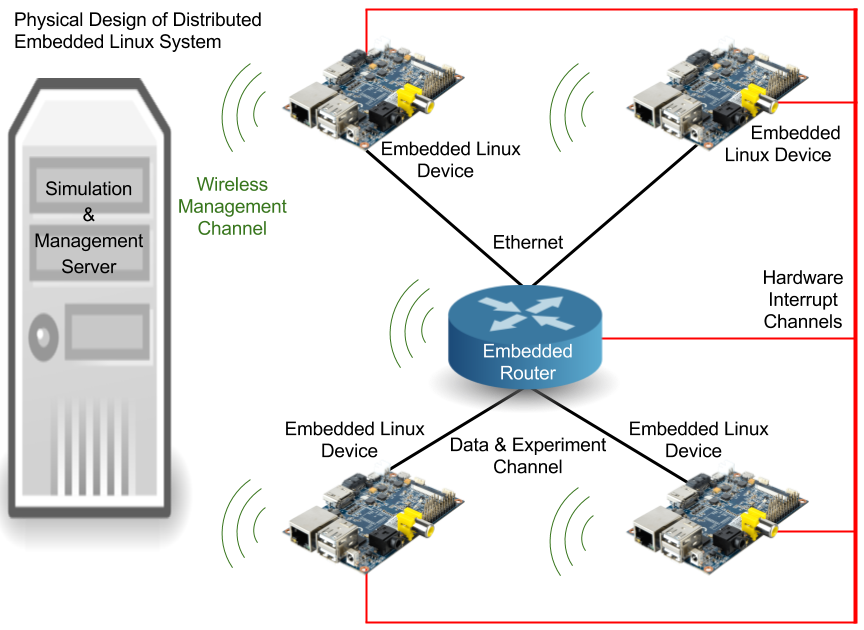
\includegraphics[scale=0.28]{Updated_architecture_emb-vt.png}
  \caption{
    Architecture of distributed system composed of 3 communication channels: Ethernet, wireless management, and direct hardware connection with general purpose and router linux hardware.
    }
\end{figure}


\section{Design}
The design of the testbed includes 2 main components: the simulation and management server, and the distributed embedded communication network system. The simulation server processes time-step simulation events and requests from the communication models while the embedded communication can run a single model or emulate multiple modules on a single device.

\subsection{Simulation and Management Server}
The simulation and management server is responsible for interfacing the electric power simulator with the distributed linux testbed. Additionally the management features require that the server have the ability to initiate processes on the embedded devices in order to kickoff experiments. For electric power simulation, the user specifies the configuration of the power circuit, power related parameters, and sensor and relay devices. Elements in the power system may have a communication presence and then are represented as models in either

\subsection{Distributed Linux System}

The distributed embedded linux system is composed of standard lightweight processors and networking devices. Figure 5 shows the architecture of the distributed system. The system runs various power models such as sensors, relays, energy storage devices which have a simulated presence in the power simulator as well as power system controllers that interact with the previous devices.

\begin{figure}
  \centering
  \label{env}
  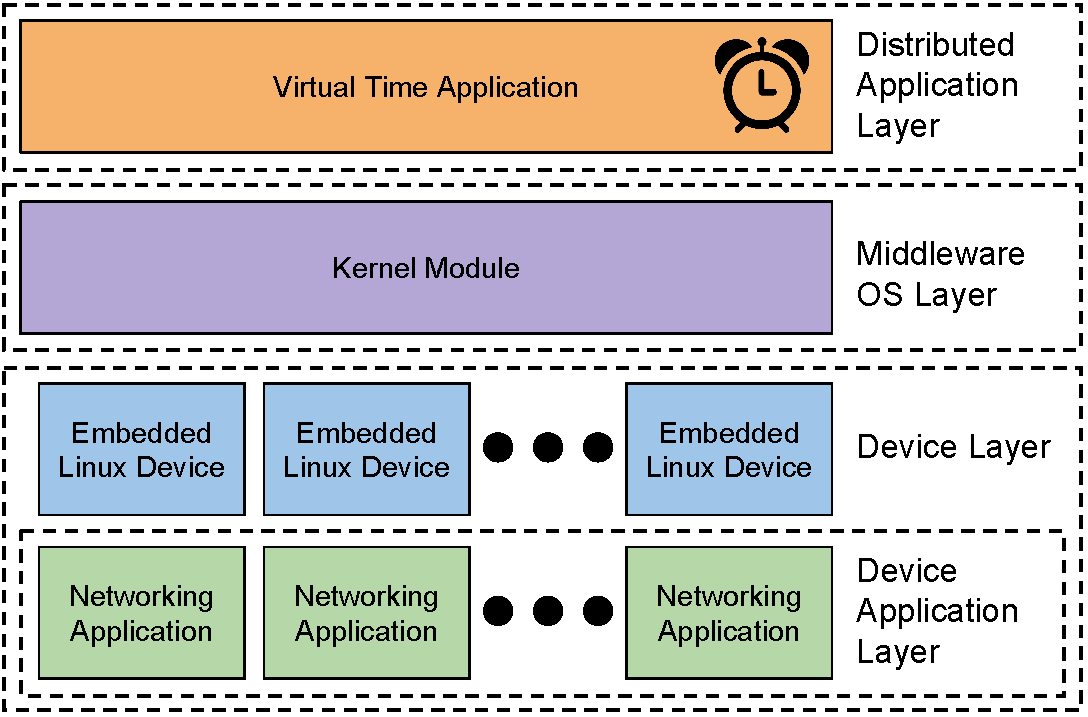
\includegraphics[scale=0.48]{Distributed_environment.pdf}
  \caption{
    The Bottom layer is the communication applications which interact during experiment. The second layer is the embedded devices which consist of commodity arm processors, and router devices. The middleware OS layer is a distributed kernel module that enables the virtual time application to run over the distributed testbed.
    }
\end{figure}

\subsection{Synchronization Challenges}
While it is possible to run electric power simulation in real-time \cite{rt-sim}, such simulators often require specialized hardware and proprietary closed software. Thus real-time simulation is infeasible for low-cost hybrid testbeds. Additionally, the real-time nature of power simulation can not account for the exchange of messages with the network system for passing messages.

Therefore due to the nature of the electric power simulator, it must run slower than real time.
This is inherently different from the way that communication systems and communication emulation systems execute.

A simulation system can be thought of a queue of events with associated time stamps.
Each event may change the state of the system, and create new events.
When a simulator progresses in time, it simply processes the next event and moves the simulation clock to the time of the event. In the case of time-step simulation, the maximum progression of time is the size of the time-step.

On the other hand, emulation and real systems' clocks progress with the real wall clock time. This difference in the systems can lead to temporal error. To remedy this problem we utilize the virtual time kernel \cite{Yan:VTS:pads15},\cite{Yan:VTM:sosr15} based off \cite{Lamps:TK:pads14} and expand it to work on Arm32 processor family. Additionally one of the major design differences is the distributed nature of our communication network.



\begin{figure}
  \centering
  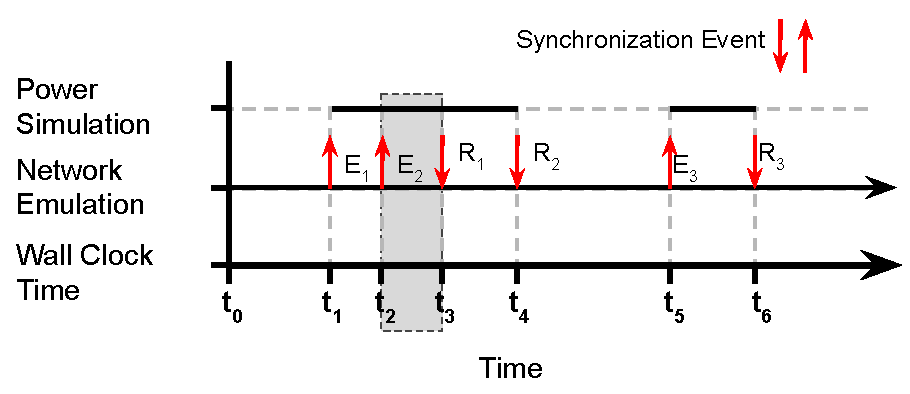
\includegraphics[scale=0.5]{no-pause-error.pdf}
  \label{sim-err}

  \caption{
    The execution of the system is shown with respect
    to the wall clock. The network (emulation) runs concurrently
    with the power simulation, and is not paused which allows
    for synchronization errors to occur, when requests arrive be-
    fore the responses are sent, i.e., $R_1$ occurs after $E_2$. The
  shaded box highlights the location of the error.}
\end{figure}

In Figure 3, there are three cross-system events ($E_i$), each
with a response ($R_i$). $E_1$ occurs before $E_2$, however, $E_2$ may
require information from $R_1$. Since the response occurs after
the second event, the global causality is violated, and thus
reduces experiment fidelity. An example of $_1$ is a request
to retrieve power flow values while $E_2$ sets the value of a
discharging battery based on the value returned previously.
Since the reply $R_1$ occurs after $E_2$ this can introduce an
error. Furthermore, such errors can be accumulated if the
simulation keeps out of synchronization with the distributed emulation.

\begin{figure}
  \centering
  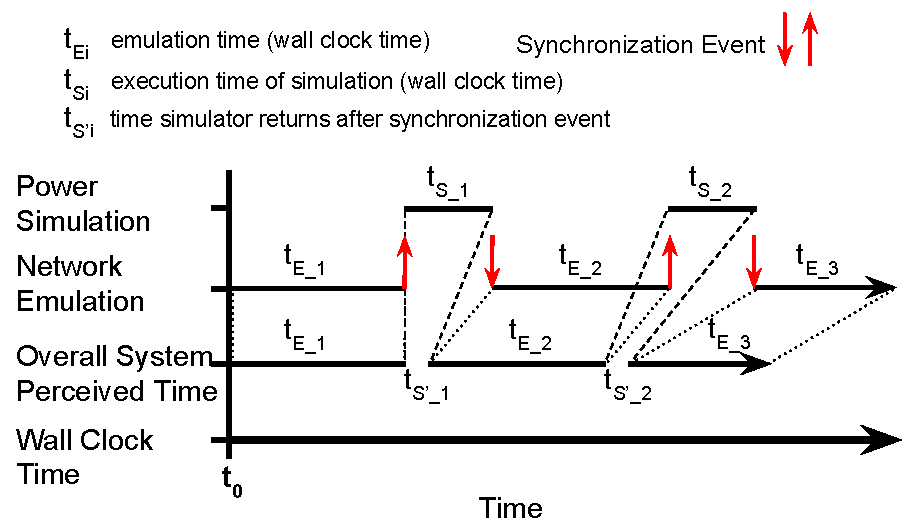
\includegraphics[scale=0.5]{wall_clock.pdf}
  \label{sim-err}

  \caption{
    The execution of the system is shown with respect
    to its own perceived time, i.e., the sum of the elapsed wall clock time or emulation
    execution time and the virtual time elapsed in simulation. The network emulation is paused
    to allow for the simulation to catch up to the emulation—
    this also ensures synchronization errors in the early example
    do not occur.
  }
\end{figure}

In order to overcome the synchronization challenges, we utilize the virtual time kernel's ability to freeze (or pause) the emulated processes clocks. The technique by which we perform the freeze and unfreeze over the distributed system is through the middleware layer that creates a unified control of virtual time over the distributed system.

\subsection{Virtual Time System}
Building on previous work by Yan \cite{Yan:VTS:pads15} we extend the virtual time kernel for distributed environments. The methods we do this by is a hardware bus that connects the devices. Communication is binary over hardware interrupts that enable the devices to indicate to each other in a distributed fashion to initiate the pausing of the virtual clocks. The synchronization algorithm is kicked off by a process that creates an event to the power simulator. Upon this time, the kernel module on the local process triggers the distributed pause using the hardware interrupt. At this time each device can freeze the required virtual clocks. When the simulator is finished processing events it places the result in the calling processes buffer and the kernel module can begin the unfreeze routine similar to the freeze one.
\begin{figure}
  \centering
  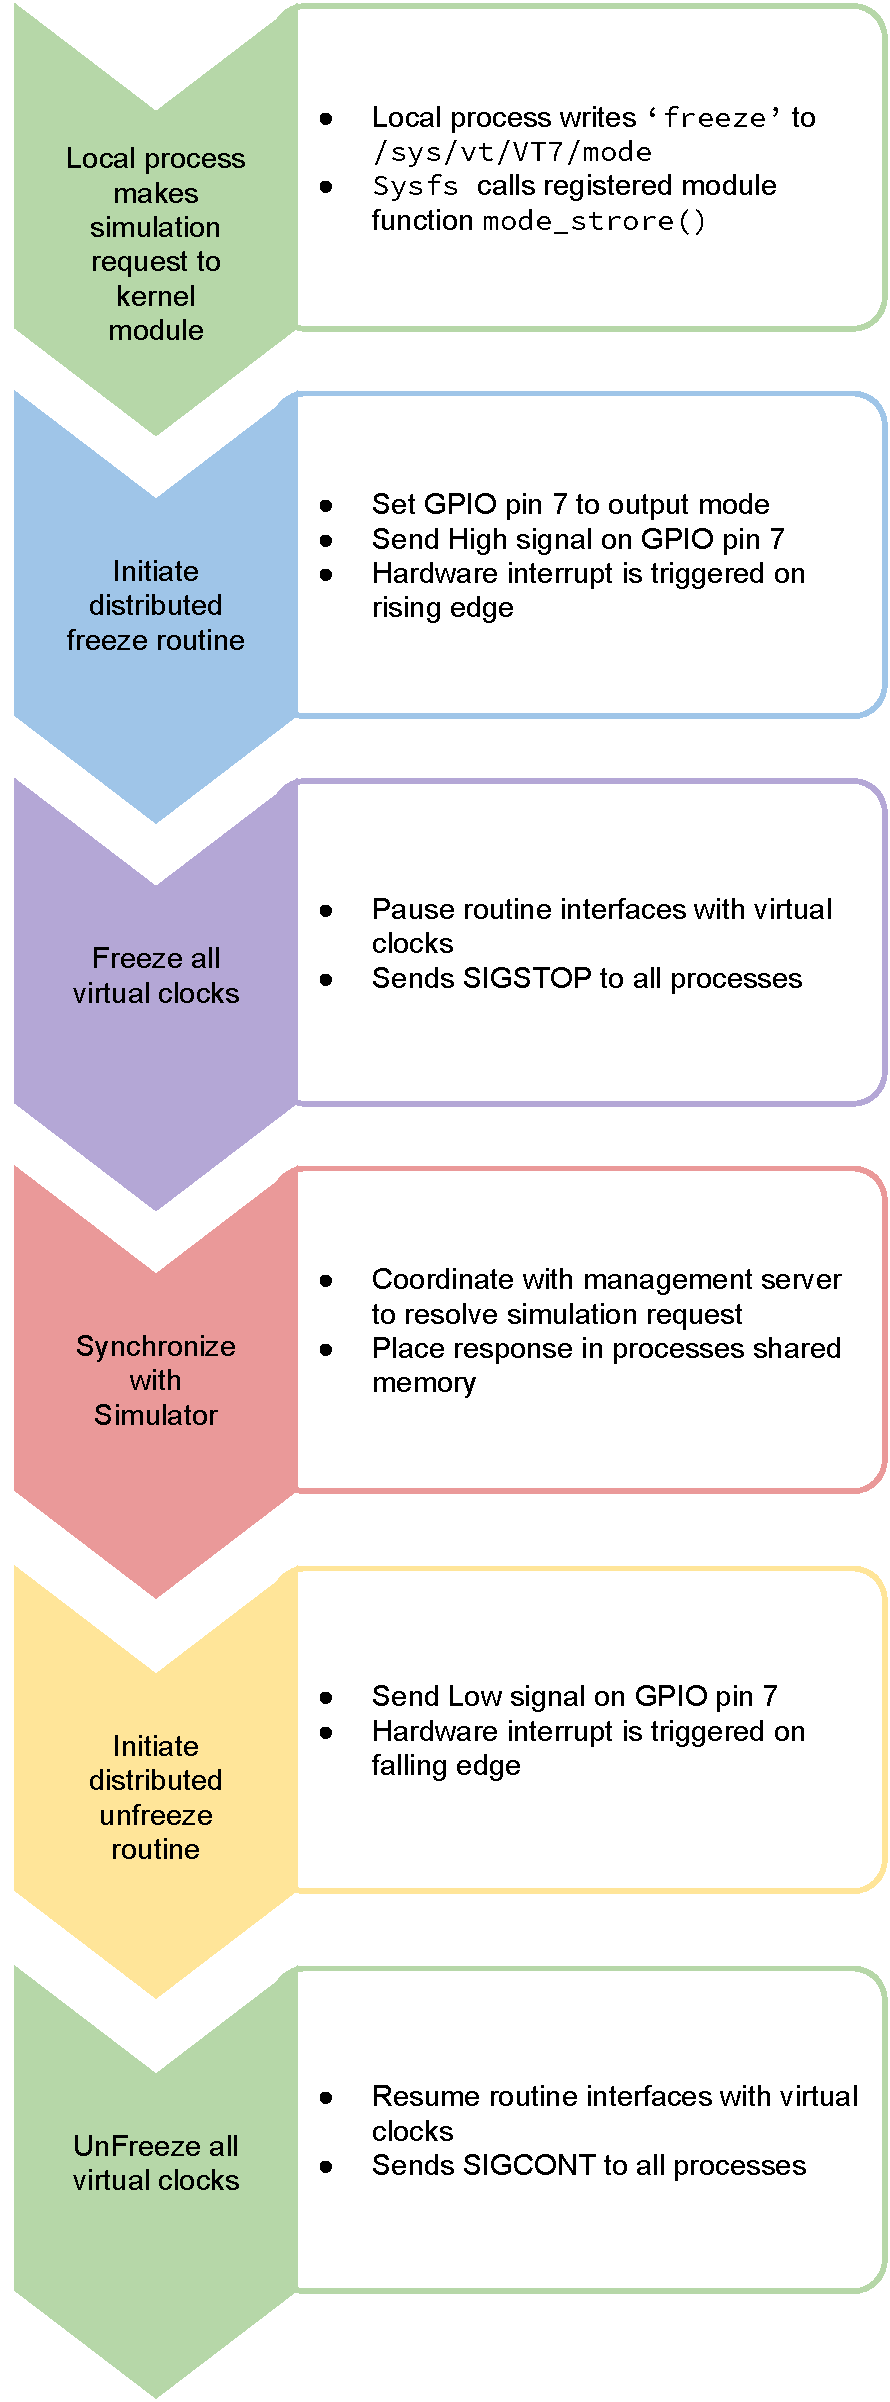
\includegraphics[scale=0.48]{Distributed_Algo.pdf}
  \caption{
    The overview of the distributed algorithm.
    }
\end{figure}

\subsection{Distributed Emulation}
\

For our testbed to model larger systems, each linux device is loaded with Mininet, a network emulator which uses lightweight linux containers to run real network applications. The number of hosts Mininet may emulate is limited by the machine's CPU.

In order for our testbed to be scalable, we enabled distributed emulation by connecting remote instances of Mininet with GRE tunnels. An emulated module emulated on device A therefore may seamlessly communicate with an emulated module on device B as if they were on the same emulated network. The fact that communication between such two modules takes place over a physical link only further increases the fidelity of the testbed. Each linux device may act as single worker in a larger emulation environment, allowing the emulation capabilities to scale with each additional device.

The design of this distributed emulation environment across hardware with physical communication channels enables our testbed to maintain fidelity and scalability. Furthermore, the integration of Mininet in our design allows us to more easily pursue future research interests surrounding SDN technologies, as SDN emulation is central to Mininet development.

\section{Implemenation}

The simulation server we utilize from our previous work DSSnet \cite{Hannon:2016}.
The testbed that we create is composed of 2 Banana Pi devices, 1 embedded router Banana Pi R1, and 2 Raspberry Pi devices all running Raspian Linux 3.04 kernel.

\subsection{Virtual Time}
Our largest contribution is the distributed interface to the virtual time module. The devices are physically connected on GPIO pins 7 and 9. Each device loads an identical kernel module \textit{emb-vt}. The module registers a hardware interrupt on both pins 7 and 9 which share the same physical bus. The module registers a low to high interrupt on one pin and a high to low interrupt on the other. The module also creates several objects in /sys/vt/VT7/ including entries to register process ids, dilation factor, and a boolean variable to trigger the freeze and unfreeze routines.
When a process triggers the freeze, the module will change its pin 7 from low power to high power causing the rest of the devices to receive the signal to their hardware interrupt. The next step is that all devices will write to their /proc/\$PID/freeze object that triggers the timekeeping to occur as per \cite{Yan:VTS:pads15}.
Essentially the kernel records the time and stores an accumulated offset in the proc file system for each process. The benefit of this approach is that each process has its own virtual clock.
When the process triggers the unfreeze, the module will change its pin 7 back to low causing the interrupt on pin 9 to occur, resuming the processes clocks.

\section{Evaluation}
In this section we evaluate the testbed's performance and overhead. It was first necessary to ensure the device clocks were synchronized and that the hardware interrupt was working as expected, i.e. with nominal delay. Device clocks are synchronized  within a single millisecond via Network Time Protocol (NTP). NTP synchronizes clocks to a remote reference time. Each clock polls these reference servers where offset and round-trip delay are calculated and clock frequencies adjusted accordingly. Results are shown below.

\begin{figure}[H]
  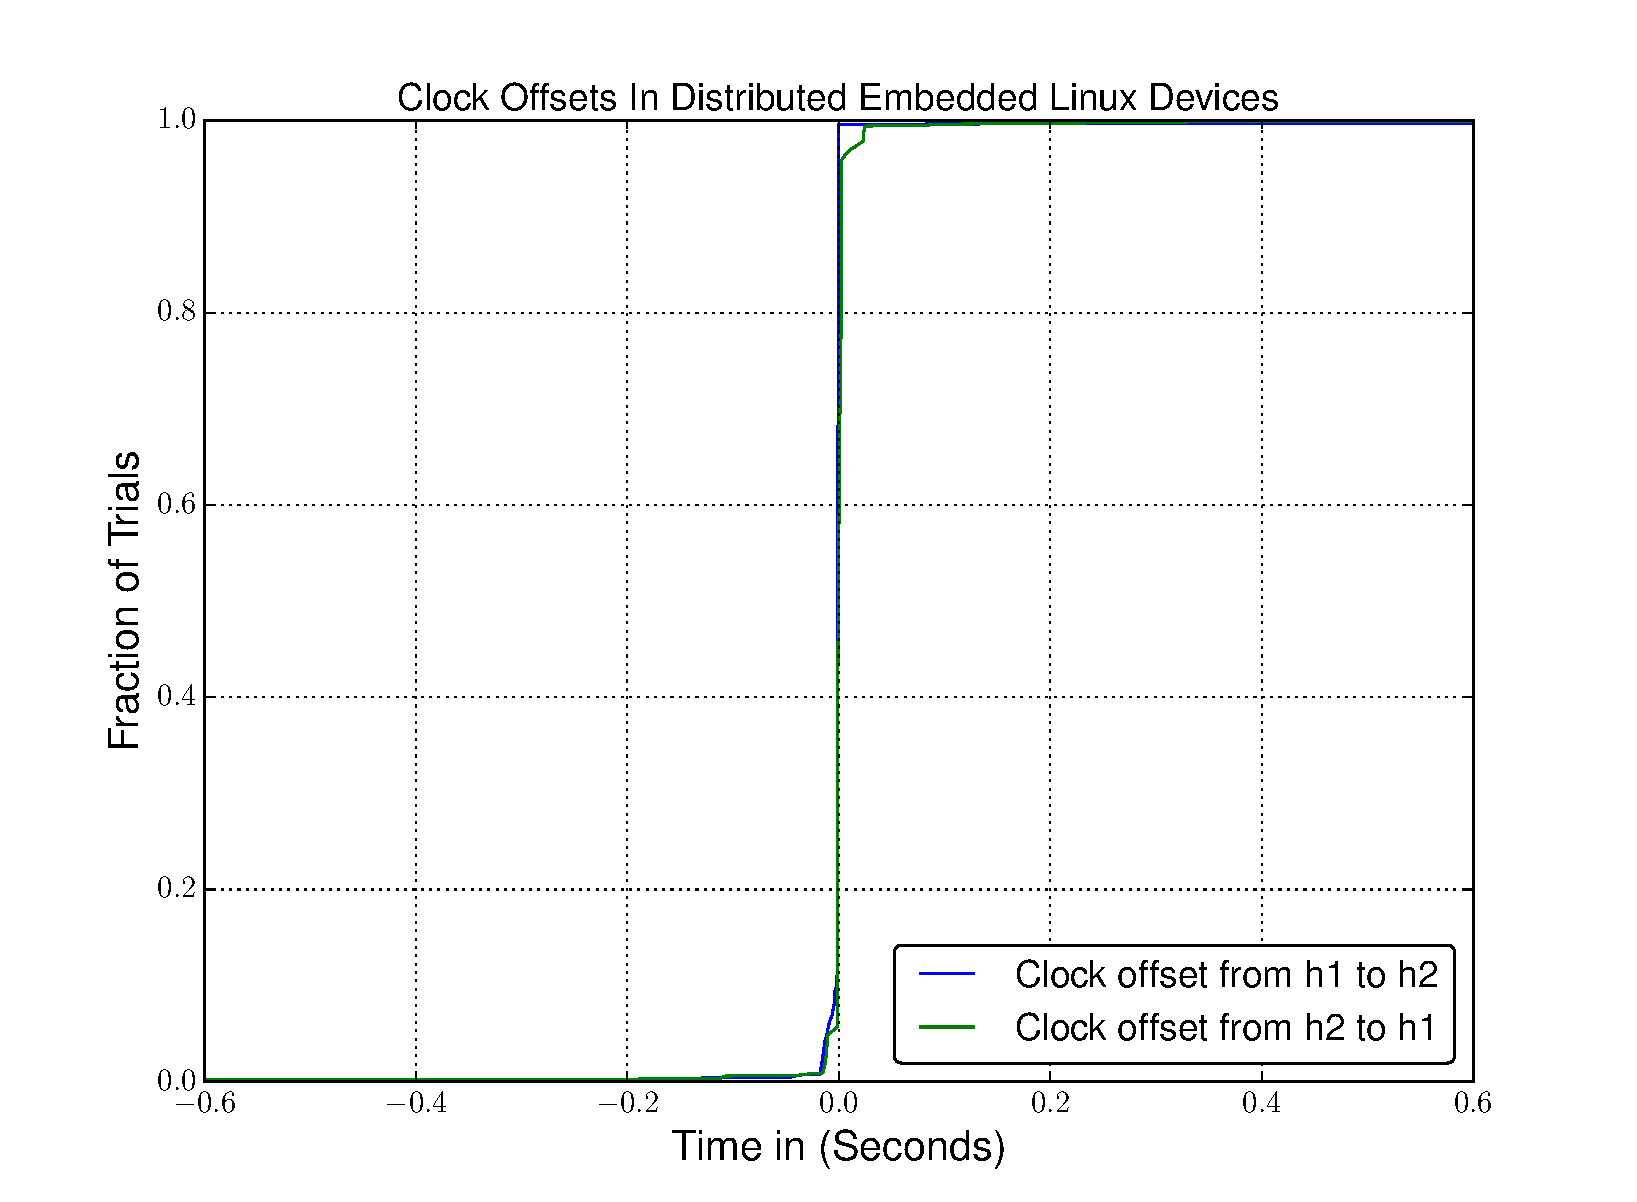
\includegraphics[scale=0.25]{clock_offset_cdf.pdf}
  \label{sim-err}

  \caption{The clock offsets CDF for two devices is shown. Device 1 timestamps and sends a hardware interrupt to device 2 and the offset is calculated with the timestamp taken upon received interrupt. Results show the clock offsets and interrupt overhead of the devices is nominal, on average less than a millisecond.
    }
\end{figure}

\begin{figure}[H]
  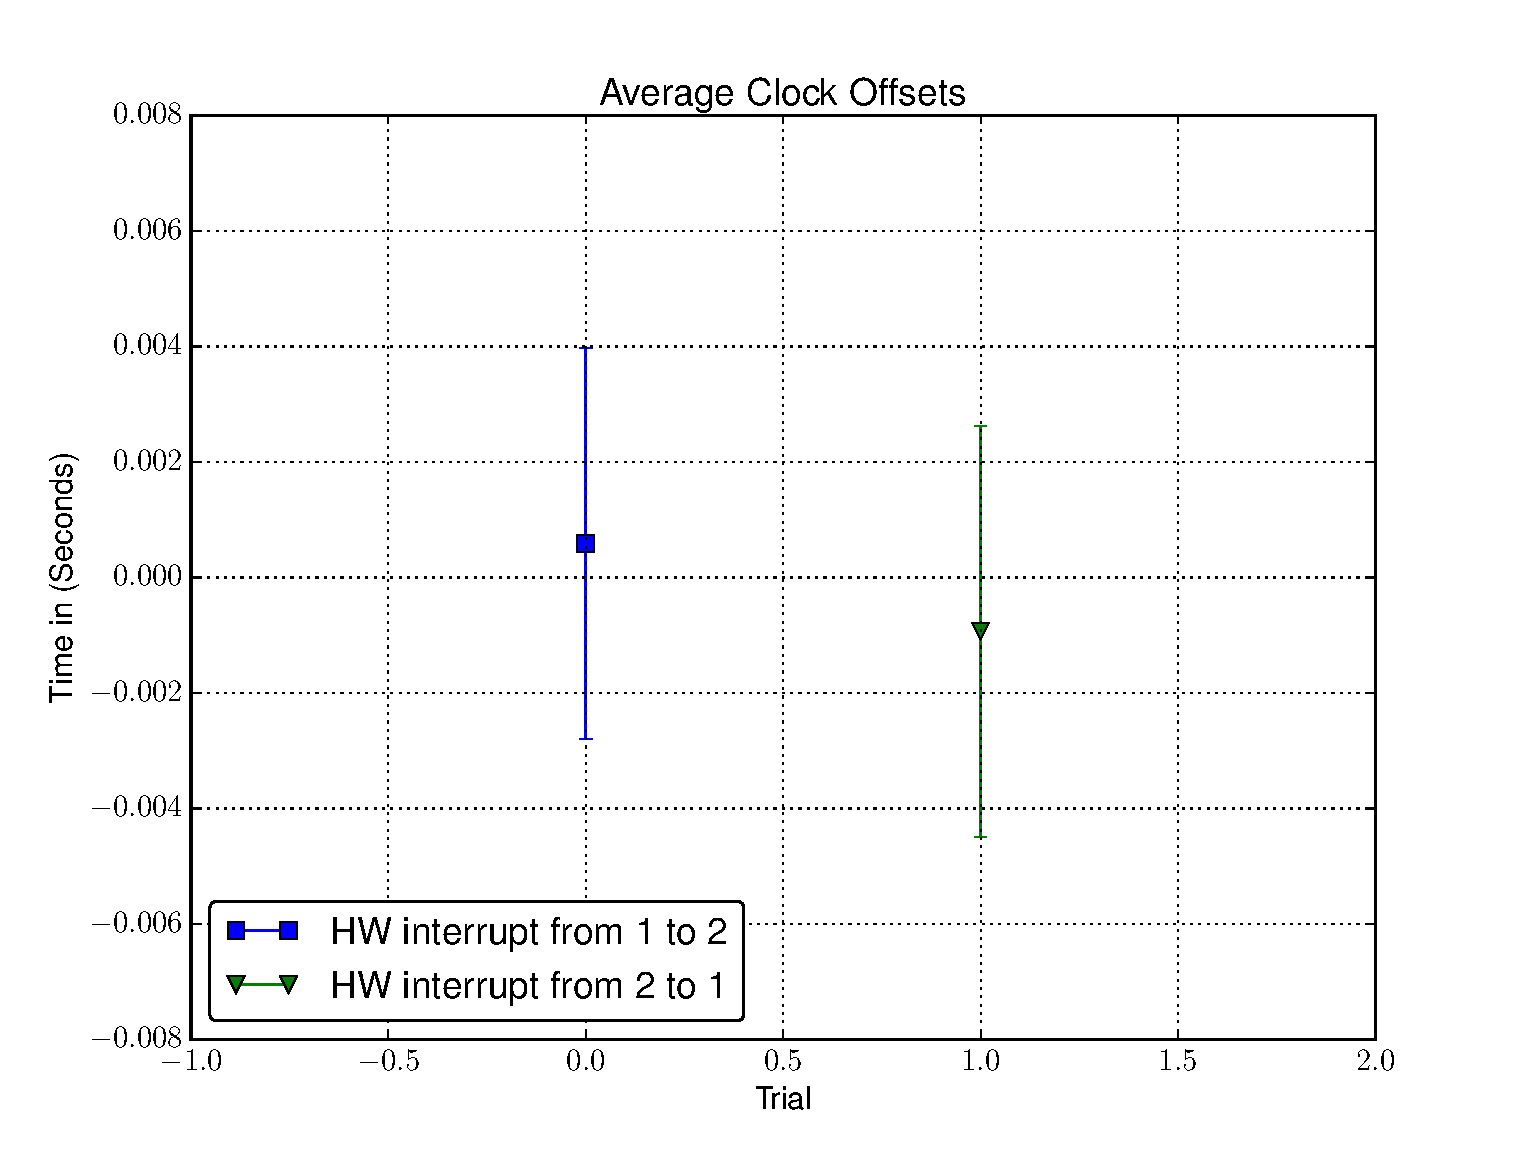
\includegraphics[scale=0.25]{clock_offset_avg.pdf}
  \label{sim-err}

  \caption{A closer look at the average and deviation of the clock offsets.
    }
\end{figure}

With the clock offset of the devices at expectantly nominal levels, correct behavior of virtual time required validation. This was done by comparing the timestamps of two processes on a single device, one of these processes being in virtual time. Two processes A and B are started in a paused state, B is put in virtual time. Every 0.5 seconds A sends a timestamped piped message to B and B records this time and its own time. Every 2 seconds B is frozen and another 2 seconds later unfrozen. In this way, when B is unfrozen it is expected that the buffered messages from A will maintain the same interval while B will have perceived no time to have passed. Results are shown below.

\begin{figure}[H]
  \includegraphics[scale=0.22]{wc_vs_vt.png}
  \label{sim-err}

  \caption{As expected, the timestamps for A grow at a linear rate, while B perceives no time to pass each time it is unfrozen. This validates the correctness several key components of the testbed, the interface to put a process in virtual time, freeze and unfreeze that process as well as the gettimeofday() system call.
    }
\end{figure}

Knowing that the key components of the testbed were in place and working as expected, the scalability of our proposed design could be tested. We found that the overhead for the freeze and unfreeze operations was on average 69.948 milliseconds with a standard deviation of 8.556 milliseconds. 

While this overhead is relatively consistent, it is well above what we expected and casts doubt into the scalability of a testbed using these specific devices. Note that given the nominal overhead of the hardware interrupt, each device undertakes this operational delay concurrently. Lowering this overhead moving forward is a primary goal for developing a truly scalable testbed.

\section{Conclusion and Future Work}
We present an distributed embedded linux device testbed, a testing platform that combines an
electrical power system simulator and real communication network and distributed emulator platform. This tesbed can be used to model and simulate power flows, communication networks, and smart grid control application, and to evaluate the effect of network applications on the smart grid. 

Our future work includes
exploring means to extract emulation lookahead to improve
the performance of this hybrid system, as well as evaluating the scalability of the testbed for large-scale experiments. 

We also plan to investigate several novel SDN
applications for microgrid security and resilience, such as context-aware intrusion detection with PMU networks. Finally to improve the performance of the virtual time system we plan to explore real-time linux operating systems including direct control over the linux scheduler.

\section{Work Distribution}
Below is an itemized list of the distribution of the main contributions. Most items were collaborative to some extent.
\\
Chris

-Hardware configuration

-Porting the virtual time kernel

-Distributed synchronization strategy and interface
\\
Neil

-Distributed emulation

-Evaluation tests and analysis

-Debugging kernel
\\
Collaborative

-Presentation

-Final Report

-Charts and figures

-Poster


\section{Acknowledgements}
Thanks to Jiaqi Yan for his origional Virtual-Time kernel source code and his assistance. Thanks to professor Lan for providing us with the knowledge of distributed algorithms and systems. Thanks to Professor Kevin Jin for his support and funding the testbed.

%
% The following two commands are all you need in the
% initial runs of your .tex file to
% produce the bibliography for the citations in your paper.
\bibliographystyle{abbrv}
\bibliography{sigproc}  % sigproc.bib is the name of the Bibliography in this case
% You must have a proper ".bib" file
%  and remember to run:
% latex bibtex latex latex
% to resolve all references
%
% ACM needs 'a single self-contained file'!
%

%\nocite{*}
%\balancecolumns % GM June 2007
% That's all folks!

%\elecappendix
%\medskip


\end{document}
